\documentclass[a4paper]{report}
\author{Jack Lipson}

% fancy headers
\usepackage{fancyhdr}
\pagestyle{fancy}

\fancyhead[LO]{Jack Lipson}
\fancyhead[RO]{\@lesson}
\fancyfoot[RO]{\thepage}
\fancyfoot[C]{\leftmark}

% basics
\usepackage[utf8]{inputenc}
\usepackage[T1]{fontenc}
\usepackage{siunitx} % e.g. \qty{1e10}{kg}
\usepackage{textcomp}
% \usepackage[dutch]{babel}
\usepackage{url}
\usepackage{hyperref}
\hypersetup{
    colorlinks,
    linkcolor={black},
    citecolor={black},
    urlcolor={blue!80!black}
}
\usepackage{graphicx}
\usepackage{float}
\usepackage{booktabs}
\usepackage{enumitem}
\usepackage{parskip}
\usepackage{emptypage}
\usepackage{subcaption}
\usepackage{multicol}
\usepackage{faktor}
\usepackage[dvipsnames,table,xcdraw]{xcolor}

% \usepackage{cmbright}


\usepackage{amsmath, amsfonts, mathtools, amsthm, amssymb}
\usepackage{mathrsfs}
\usepackage{cancel}
\usepackage{bm}
\newcommand\N{\ensuremath{\mathbb{N}}}
\newcommand\R{\ensuremath{\mathbb{R}}}
\newcommand\Z{\ensuremath{\mathbb{Z}}}
\renewcommand\O{\ensuremath{\emptyset}}
\newcommand\Q{\ensuremath{\mathbb{Q}}}
\newcommand\C{\ensuremath{\mathbb{C}}}

\DeclareMathOperator{\sgn}{sgn}
\DeclareMathOperator{\Ker}{ker}
\DeclareMathOperator{\im}{Im}
\DeclareMathOperator{\degree}{\!^{\circ}\!}

\usepackage{systeme}
\let\svlim\lim\def\lim{\svlim\limits}
\let\implies\Rightarrow
\let\impliedby\Leftarrow
\let\iff\Leftrightarrow
\let\epsilon\varepsilon
\let\vec\mathbf
\let\mean\overline{}

\usepackage{stmaryrd} % for \lightning
\newcommand\contra{\scalebox{1.1}{$\lightning$}}


% horizontal rule
\newcommand\hr{
    \noindent\rule[0.5ex]{\linewidth}{0.5pt}
}

% hide parts
\newcommand\hide[1]{}

% tikz
\usepackage{tikz}
\usepackage{tikz-cd}
\usetikzlibrary{intersections, angles, quotes, calc, positioning}
\usetikzlibrary{arrows.meta}
\usepackage{pgfplots}
\pgfplotsset{compat=1.13}


\tikzset{
    force/.style={thick, {Circle[length=2pt]}-stealth, shorten <=-1pt}
}

% theorems
\makeatother
\usepackage{thmtools}
\usepackage[framemethod=TikZ]{mdframed}
\mdfsetup{skipabove=1em,skipbelow=0em}


\theoremstyle{definition}

\declaretheoremstyle[
    headfont=\bfseries\sffamily\color{ForestGreen!70!black}, bodyfont=\normalfont,
    mdframed={
        linewidth=2pt,
        rightline=false, topline=false, bottomline=false,
        linecolor=ForestGreen, backgroundcolor=ForestGreen!5,
    }
]{thmgreenbox}

\declaretheoremstyle[
    headfont=\bfseries\sffamily\color{NavyBlue!70!black}, bodyfont=\normalfont,
    mdframed={
        linewidth=2pt,
        rightline=false, topline=false, bottomline=false,
        linecolor=NavyBlue, backgroundcolor=NavyBlue!5,
    }
]{thmbluebox}

\declaretheoremstyle[
    headfont=\bfseries\sffamily\color{NavyBlue!70!black}, bodyfont=\normalfont,
    mdframed={
        linewidth=2pt,
        rightline=false, topline=false, bottomline=false,
        linecolor=NavyBlue
    }
]{thmblueline}

\declaretheoremstyle[
    headfont=\bfseries\sffamily\color{RawSienna!70!black}, bodyfont=\normalfont,
    mdframed={
        linewidth=2pt,
        rightline=false, topline=false, bottomline=false,
        linecolor=RawSienna, backgroundcolor=RawSienna!5,
    }
]{thmredbox}

\declaretheoremstyle[
    headfont=\bfseries\sffamily\color{RawSienna!70!black}, bodyfont=\normalfont,
    numbered=no,
    mdframed={
        linewidth=2pt,
        rightline=false, topline=false, bottomline=false,
        linecolor=RawSienna, backgroundcolor=RawSienna!1,
    },
    qed=\qedsymbol
]{thmproofbox}

\declaretheoremstyle[
    headfont=\bfseries\sffamily\color{NavyBlue!70!black}, bodyfont=\normalfont,
    numbered=no,
    mdframed={
        linewidth=2pt,
        rightline=false, topline=false, bottomline=false,
        linecolor=NavyBlue, backgroundcolor=NavyBlue!1,
    },
]{thmexplanationbox}

\declaretheorem[style=thmgreenbox, name=Definition]{definition}
\declaretheorem[style=thmbluebox, numbered=no, name=Example]{example}
\declaretheorem[style=thmredbox, name=Proposition]{proposition}
\declaretheorem[style=thmredbox, name=Theorem]{theorem}
\declaretheorem[style=thmredbox, name=Lemma]{lemma}
\declaretheorem[style=thmredbox, numbered=no, name=Corollary]{corollary}
\declaretheorem[style=thmblueline, numbered=no, name=Remark]{remark}
\declaretheorem[style=thmblueline, numbered=no, name=Note]{note}

\declaretheorem[style=thmproofbox, name=Proof]{replacementproof}
\renewenvironment{proof}[1][\proofname]{\vspace{-10pt}\begin{replacementproof}}{\end{replacementproof}}

\declaretheorem[style=thmexplanationbox, name=Explanation]{tmpexplanation}
\newenvironment{explanation}[1][]{\vspace{-10pt}\begin{tmpexplanation}}{\end{tmpexplanation}}

% http://tex.stackexchange.com/questions/22119/how-can-i-change-the-spacing-before-theorems-with-amsthm
\makeatletter
% \def\thm@space@setup{%
%   \thm@preskip=\parskip \thm@postskip=0pt
% }

\def\@lesson{}
\newcommand{\lesson}[3]{
    \ifthenelse{\isempty{#3}}{%
        \def\@lesson{Lecture #1}%
    }{%
        \def\@lesson{Lecture #1: #3}%
    }%
    \subsection*{\@lesson}
    \marginpar{\small\textsf{#2}}
}

\makeatother

% notes
\usepackage{todonotes}
\usepackage{tcolorbox}

\tcbuselibrary{breakable}
\newenvironment{verbetering}{\begin{tcolorbox}[
    arc=0mm,
    colback=white,
    colframe=green!60!black,
    title=Opmerking,
    fonttitle=\sffamily,
    breakable
]}{\end{tcolorbox}}

\newenvironment{noot}[1]{\begin{tcolorbox}[
    arc=0mm,
    colback=white,
    colframe=white!60!black,
    title=#1,
    fonttitle=\sffamily,
    breakable
]}{\end{tcolorbox}}

% figure support
\usepackage{import}
\usepackage{xifthen}
\pdfminorversion=7
\usepackage{pdfpages}
\usepackage{transparent}
\newcommand{\incfig}[1]{%
    \def\svgwidth{\columnwidth}
    \import{./figures/}{#1.pdf_tex}
}

%binary op tables
\usepackage{array, makecell}

\newcommand\thickvrule{\vrule width 1pt}
\newcommand\thickhrule{\Xhline{1pt}}

% %http://tex.stackexchange.com/questions/76273/multiple-pdfs-with-page-group-included-in-a-single-page-warning
\pdfsuppresswarningpagegroup=1

\title{Elementary Algebraic Topology}
\begin{document}
    \usetikzlibrary{decorations.markings,arrows.meta,bending, patterns, math}

\subsection*{Page 183, Problem 11 (ab) (Worked with David LaRoche)}
\vspace{15pt}
\begin{proof}
    \vspace{-10pt}
    \begin{enumerate}[label = (\alph*)]
        \item Join together three copies of the boundary of a triangle at a single vertex as shown below:
        \begin{center} \;\begin{tikzpicture}
                \tikzset{->-/.style={decoration={
                markings,
                mark=at position #1 with {\arrow{<}}},postaction={decorate}}, ->>-/.style={decoration={
                markings,
                mark=at position #1 with {\arrow{>>}}},postaction={decorate}}}
                
                \node[left = 2cm] (0,0) {$K$};
                \node[below = .25cm] (0,0) {$v_6$};
                \foreach \t/\x in {0/0, 120/2, 240/4}{
                    \tikzmath{\a = \x; \b = int(\x + 1);}
                    \draw[white] (0,0) -- (\t+60:1.2) node[black] {$v_\a$} -- (\t+120:1.2) node[black] {$v_\b$} -- cycle;
                    \draw[thick] (0,0) -- (\t+60:1) -- (\t+120:1) -- cycle;}
        \end{tikzpicture} \end{center}
        $|K|$ is connected so $$H_0(K) = \Z^1 \quad \text{[Theorem 8.2]}.$$ $K$ has fundamental group of a 3-bouquet $F_3$ generated by $z_1 = (v_6v_1) + (v_1v_0) + (v_0v_6)$, $z_2 = (v_6v_5) + (v_5v_4) + (v_4v_6)$, and $z_3 = (v_6v_3) + (v_3v_2) + (v_2v_6).$ Thus, its abelianization \[\langle z_1, z_2, z_3 \mid z_1z_2z_1^{-1}z_2^{-1}, z_1z_3z_1^{-1}z_3^{-1}, z_2z_3z_2^{-1}z_3^{-1} = e \rangle\] is equal to $$H_1(K) \cong \Z^3\quad \text{[Theorem 8.3]}.$$ There are no 2 - or higher - simplexes so $B_{\geq 2}(K), Z_{\geq 2}(K) = \{0\}$ and $$H_q(K) = \{0\} \quad q \geq 2.$$

        \item We can glue two hollow tetrahedra along an edge to get the following:
        \begin{center}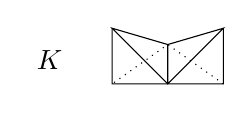
\begin{tikzpicture}
            \tikzset{->-/.style={decoration={
            markings,
            mark=at position #1 with {\arrow{<}}},postaction={decorate}}, ->>-/.style={decoration={
            markings,
            mark=at position #1 with {\arrow{>>}}},postaction={decorate}}}
            
            \node[xshift = -1.5cm, yshift = .3cm] (0,0) {$K$};
            \draw (0,0) -- (45:1) -- (90:.5) -- (135:1) -- cycle -- (90:.5);
            \draw (0,0) -- (0:.707) -- (45:1);
            \draw (0,0) -- (180:.707) -- (135:1);
            \draw[dotted] (0:.707) -- (90:.5) -- (180:.707);
        \end{tikzpicture} \end{center}
        $|K|$ is connected so $$H_0(K) = \Z^1 \quad \text{[Theorem 8.2]}.$$ Note that each empty tetrahedra is homeomorphic to $S^2$ so they have the same homotopy type. Because they're path-connected, they have isomorphic fundamental groups $\{e\}$. Now, by Van Kampen's theorem, $K$ has the same fundamental group as the one point union of 2-spheres and thus has fundamental group equal to the free product of each trivial group which is itself the trivial group. Thus, $\pi_1(K)$'s abelianization gives $$H_1(K) = \{0\}\quad \text{[Theorem 8.3]}.$$ There are no complexes of dimension 3 or greater so $B_2(K)$, $B_3(K)$, $\cdots = \{0\}$ and $Z_3(K), Z_4(K), \cdots = \{0\}$. We can therefore show $H_2(K) = Z_2(K)/\{0\} = \text{Ker } \partial\colon C_{2}(K)\to C_{1}(K) \cong \Z^2$ as follows. Pick any 2-simplex to start. To annihilate the boundary of any 2-chain starting at this triangle, we MUST orient it compatibly with another 2-simplex on the same tetrahedron in order to kill their shared edge. This requires another 2-simplex on the same tetrahedron by the same argument and then the last one, all on one tetrahedron. This has already killed the boundary so its clear any 2-cycle can be decomposed into scalar multiples of these isolated 2-cycles on each tetrahedredon. Therefore, they together generate $Z(K)$. Addition of these cycles is commutative so the abelianization gives $\Z(K) \cong \Z^2$. Thus, $$H_2(K) = Z_2(K)/\{0\} \cong \Z^2.$$ Given what we said about $Z_3(K), Z_4(K), \cdots$ and $B_3(K), B_4(K), \cdots$, $$H_q(K) = \{0\} \quad q \geq 3.$$
    \end{enumerate}
\end{proof}

\subsection*{Page 183, Problem 13}
\vspace{15pt}
\begin{proof}
    \vspace{-10pt}
    Take any (path-connected) graph $\Gamma$ with maximal tree $T$. $G(\Gamma,T)$ by construction includes only the generators $g_{ij}$ ($i <j$) of edges of $\Gamma-T$ each `representing' exactly one non-2-simplex triangle (a triangle made of 3 1-simplices which is not filled in). Recall every such triangle also has only this generator. $T$ is clearly contractible and can be thought of as a single vertex from which each edge generator is independently attached so that $G(\Gamma, T)$ is isomorphic to the free group on $n$ generators where $n$ is the number of such edges. (Recall specifically there are no relations in $G(\Gamma, T)$ as $T$ is maximal and an edge path contained entirely within $T$ can always be found from the basepoint to some generator and back implying the generators are indpendent.) Last, $\Gamma$ is path-connected so $G(\Gamma,T)$ is isomorphic to $\pi_1(\Gamma, v)$ regardless of choice of $v$. 
    
    This same result can also be achieved through repeatedly applying Van Kampen's theorem on $T$ and one empty triangle at a time which would each time give just the generating loop of that triangle with the single relation that that loop 0 times is the identity, i.e. the trivial relation and therefore a free group on $\beta_1$ generators.

    The homeomorphic reduction of 2-simplices first into one of their respective line-segment components and then all of $T$'s `spikes' down into just one point leaving only empty triangles implies $\Gamma$ shares the exact homotopy type as a bouquet of circles. This also implies their isomorphic fundamental groups.
        
    Now by Theorem 8.3, the abelianization of $F_n$ gives $\overbrace{\Z \oplus \cdots \oplus \Z}^{n \text{ times}} \cong \Z^n$ as the first homology group of $\Gamma$. $H_1(\Gamma)$ has no torsion element so the first Betti number of $\Gamma$ is the rank of $\Z^n$, i.e. n, i.e. the number of not-filled-in triangles in the graph = $\beta_1$. 

\end{proof}

\subsection*{Page 188, Problem 20}
\vspace{15pt}
\begin{proof}
    \vspace{-10pt}
    Take chain maps $\phi\colon C(K)\to C(L)$, $\psi\colon C(L)\to C(M)$. Because $\partial\circ\phi_q = \phi_{q-1}\circ\partial$ and $\partial\circ\psi_q = \psi_{q-1}\circ\partial$, we know that $$\partial\circ(\psi_q\circ\phi_q) = (\partial\circ\psi_q)\circ\phi_q=(\psi_{q-1}\circ\partial)\circ\phi_{q}=(\psi_{q-1}\circ\phi_{q-1})\circ\partial.$$
    (Generically, we can show our induced map is well-defined via the following. For normal subgroups $N \vartriangleleft G, M \vartriangleleft H$ and $f\colon G\to H$, if $f(N) \subseteq M$ then $f_*\colon G/N \to H/M$ is well-defined as for any cosets $g_1 + N = g_2 + N$, $f(g_1) + M = f(g_1) + f(N) + M = f(g_1 + N) + M = f_*(g_1 + N) = f_*(g_2+N) = f(g_2 + N) + M = f(g_2) + f(N) + f(M) = f(g_2) + M$. This is trivially a homomorphism too.)

    Thus, to show $\psi\circ\phi$ induces a homomorphism $(\psi\circ\phi)_{*}\colon H_q(K)\to H_q(M)$, we need only show $\psi_q\circ\phi_q(Z_q(K)) \subseteq Z_q(M)$ and $\psi_q\circ\phi_q(B_q(K)) \subseteq B_q(M)$. This is implied (via the proof on page 185) by the fact that both $\psi, \phi$ are chain maps and therefore \begin{align*}\psi_q\circ\phi_q(Z_q(K))\subseteq \psi_q(Z_q(L))\subseteq Z_q(M),\\ \psi_q\circ\phi_q(B_q(K))\subseteq \psi_q(B_q(L))\subseteq B_q(M).\end{align*} Thus, $\psi\circ\phi$ is a chain map and by the above containments, for any $z \in Z_q(K)$, we get $(\psi\circ\phi)_*(z+B_q(K)) = (\psi\circ\phi)(z + B_q(K)) + B_q(M) = (\psi\circ\phi)(z) + \psi\circ\phi(B_q(K)) + B_q(M) = (\psi\circ\phi)(z) + B_q(M) = (\psi\circ\phi)(z) + \psi(B_q(L)) + B_q(M) = \psi(\phi(z) + B_q(L)) + B_q(M) = \psi_*(\phi(z) + B_q(L)) = \psi_*(\phi(z) + \phi(B_q(K)) + B_q(L)) = \psi_*(\phi(z + B_q(K)) + B_q(L)) = \psi_*(\phi_*(z+B_q(K))) = \psi_*\circ\phi_*(z+B_q(K))$. $z$ is arbitrary so $(\psi\circ\phi)_* = \psi_*\circ\phi_*$.
\end{proof}

\subsection*{Page 192, Problem 25}
\vspace{15pt}
\begin{proof}
    \vspace{-10pt}
    Take similicial maps $s,t\colon|K|\to|L|$. Suppose there exists a homomorphism $d_q\colon C_q(K)\to C_{q+1}(L)$ for all $q$ so that $$d_{q-1}\partial + \partial d_q = t-s\colon C_q(K)\to C_{q+1}(L).$$ Then for any $z \in Z_q(K)$, $\partial(z) = 0$ and $d_q(z) \in C_{q+1}(L) \implies \partial d_q(z) \in B_q(L)$. This means $t(z) - s(z) = d_{q-1}\partial(z) + \partial(d_q(z)) = 0 + \partial d_q(z) \in B_q(L)$ and consequently that $t_*(z) - s_*(z) = [0]$ so finally $t_*(z) = s_*(z)$ for all $z$. Thefore $s,t$ induce the same homomorphism $s_* = t_*\colon H_q(K) \to H_q(L)$.
\end{proof}
    % \chapter{Kinetic Theory of Gases}

\section{The Ideal Gas Law and the Molecular Interpreation of Temperature}

\begin{definition}[Kinetic Theory]
    The analysis of matter in terms of atoms in continuous random motion is called \emph{kinetic theory}.
\end{definition}
\begin{proposition}[Postulates of Kinetic Theory]
    Under these conditions describing an 'ideal gas', real gases follow the ideal gas law quite closely. 
    \begin{enumerate}
        \item There are a large number, $N$, of molecules, each of mass $m$, moving in random directions with a variety of speeds.
        \item The molecules are, on average, far apart from one another. I.e. their average separation is much greater than their diameter.
        \item The molecules obey the laws of classical mechanics and only interact when they collide s.t. the potential energy relating to attractive forces between them is much weaker than the kinetic energy.
        \item Collisions with another molecule or the wall of the vessel are perfectly elastic and of very short duration relative to time between collisions.
    \end{enumerate}
\end{proposition}
\begin{proposition}[Temperature to Average Kinetic Energy of Molecules]
    The average translational kinetic energy of molecules in random motion in an ideal gas is directly proportional to the absolute temperature of the gas. In other words, $\overline{K} = \frac{1}{2}m\overline{v^2} = \frac{3}{2}kT$.
\end{proposition}
\begin{proof}
    Take a box of length $\ell$ and ends of area $A$ filled with an ideal gas. Focus on a single molecule of mass $m$'s collision with one wall. Newton's 2nd and 3rd laws tell us a force $F = \frac{dp}{dt}$ is exerted on the molecule. Because collisions are elastic, its velocity $v_x$ is equal in magnitude so $\Delta p = 2mv_x$. If the molecule takes time $\Delta t$ to travel $2\ell$ to the other wall and back, $F = \frac{\Delta (mv)}{\Delta t} = \frac{2mv_x}{2\ell/v_x} = \frac{m{v_x}^2}{\ell}$. Recall that although the particle may collide with the tops and sides of the container, its $x$ component doesn't change and neither does its momentum.

    We can average the force on a wall due to all the $N$ molecules in the box by $F = \frac{m}{\ell} (v_{x1}^2 + v_{x2}^2 + \cdots + v_{xN}^2)$. Averaging, $\overline{v_x^2} = \frac{v_{x1}^2 + v_{x2}^2 + \cdots + v_{xN}^2}{N}$ s.t. $F = \frac{m}{\ell} N \overline{v_x^2}$. Because $v^2 = v_x^2 + v_y^2 + v_z^2 \simeq 3v_x^2$, we let $F = \frac{m}{l}\frac{N\overline{v^2}}{3}$. Thus, the pressure on the wall is $P = \frac{F}{A} = \frac{1}{3} \frac{Nm\overline{v^2}}{A\ell} = \frac{1}{3}\frac{Nm\overline{v^2}}{V} \implies PV = \frac{2}{3}N(\frac{1}{2}m\overline{v^2})$. From the ideal gas law $PV = NkT$, such that $\frac{3}{2}kT = \frac{1}{2}(m\overline{v^2}) = \overline{KE}$. 
\end{proof}
\begin{definition}[Thermal Motion]
    This definition explains the relationship between temperature as a measure of motion of molecules such that random motion of a gas is sometimes called \emph{thermal motion}.
\end{definition}
\begin{definition}[Root-Mean-Square Speed $v_{rms}$]
    To calculate how fast moleciles molecules move on average in an ideal gas, we can derive the \emph{root-mean-square speed} $v_{rms} = \sqrt{\overline{v^2}} = \sqrt{\frac{3kT}{m}}$.
\end{definition}
\begin{remark}
    It's noteworthy that the average speed $\overline{v} \neq v_{rms}$ necessarily. In fact, for an ideal gas, they differ by about 8\%.
\end{remark}
\begin{note}
    $\overline{KE} = \frac{3}{2} kT$ tells us as $T \to 0$, $\overline{KE} \to 0$. However, modern quantum theory tells us this is not true and kinetic energy appraoches a small nonzero minimum.
\end{note}

\section{Distribution of Molecular Speeds}

\begin{definition}[Maxwell Distribution of Speeds]
    In 1859, James Maxwell worked out a formula for the most probable distribution of speeds in a gas with $N$ molecules, that is $$f(v) = 4\pi N(\frac{m}{2\pi kT})^{\frac{3}{2}}v^2e^{-\frac{1}{2}\frac{mv^2}{kT}},$$ where $f(v)dv$ represents the number of molecules that have speeds between $v$ and $v+dv$ such that $\int_0^\infty f(v)dv = N$.
\end{definition}
\begin{definition}[Activation Energy]
    Two molecules may chemically react only if their kinetic energy is great enough to partially penetrate each other. This minimum energy is called \emph{activation energy}. The rate of a chemical reaction is proportional to the number of molecules with energy greater than $E_A$ such that rates increase rapidly with increased temperature.
\end{definition}
\begin{example}[Determining $\mean{v} \text{ and} \vec{v_p}$]
    To find the average speed $\mean{v}$, we must integrate over the product of $v$ and the number $f(v)dv$ which have speed $v$ and divide by $N$ the number of molecules. Thus, $\mean{v} = \frac{\int_0^\infty vf(v)dv}{N} = 4\pi(\frac{m}{2\pi k T})^\frac{3}{2} \int_0^\infty v^3 e^{-\frac{1}{2}\frac{mv^2}{kT}}dv = 4\pi(\frac{m}{2\pi k T})^\frac{3}{2} (\frac{2k^2 T^2}{m}) = \sqrt{\frac{8}{\pi}\frac{kT}{m}}$.

    To find the most probable speed, we need simply find when the slope is $0$ such that $\frac{df(v)}{dv} = 4\pi N(\frac{m}{2\pi k T})^\frac{3}{2}(2ve^{-\frac{mv^2}{2kT}} - \frac{2mv^3}{2kT}e^{-\frac{mv^2}{2kT}})=0$. Solving for $v$ gives $v_p = \sqrt{\frac{2kT}{m}}$.
\end{example}
\begin{note}
    In summary, $$v_p \approx 1.41 \sqrt{\frac{kT}{m}}, \quad \mean{v} \approx 1.60 \sqrt{\frac{kT}{m}}, \quad v_{rms} \approx 1.73 \sqrt{\frac{kT}{m}}.$$
\end{note}

\section{Real Gases and Changes of Phase}

\ ...
\end{document}

% Green - definition
% Blue - eg, remark, note
% red - proposition, theorem, lemma, corollary
% Blue adjacent - explanation
% Red adjacent - proof

% \hide{whatever!}
% \hr inserts horizontal rule
% \contra inserts lightning symbol for contradiction
% \imples, impliedby, iff
% \cancel
% \N,R,Z,0,Q,C
% \lesson{lesson number, lesson datetime, lesson title}
% \todo[]{add a note this way}